\section{Concept Drift Types}
\label{sec:background_concept_drift_types}
Concept drift is commonly categorized into four types, as illustrated in Fig. \ref{fig:concept-drift-types}. In Types 1-3, the focus of research on concept drift adaptation revolves around minimizing the drop in accuracy and achieving the fastest recovery rate during the transformation process of concepts. Conversely, Type 4 drift delves into leveraging historical concepts, emphasizing the identification of the best-matched historical concepts within the shortest time frame when a new concept emerges—whether suddenly, incrementally, or gradually. To illuminate the distinctions between these types, \cite{losing2016knn} introduces the term "intermediate concept" to describe the transitional phases between concepts. As noted by \cite{liu2018making}, concept drift may not only occur at a precise timestamp but may also extend over a prolonged period. Consequently, intermediate concepts may emerge during the transformation, representing a blend of the starting and ending concepts in the case of incremental drift or embodying one of the starting or ending concepts, as observed in gradual drift. Understanding these intermediate concepts is essential for comprehending  the nuanced dynamics of concept drift during transitions from one state to another.
 
\begin{figure}[!ht]
    \centering
    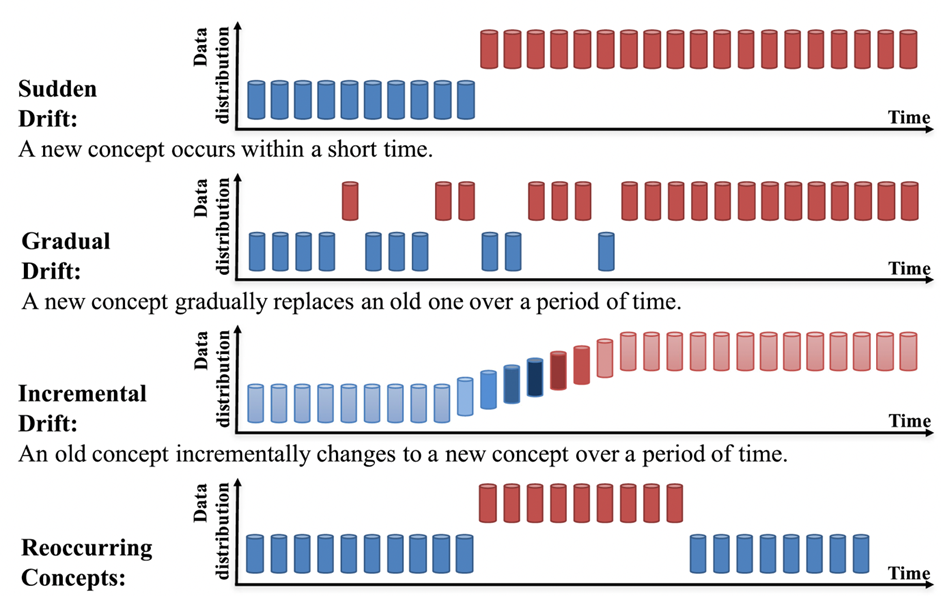
\includegraphics[width=1.0\textwidth]{2_Background/figures/concept_drift_types.png}
    \caption{Types of concept drift. \\ \textcolor{gray}{\fontsize{10}{0}\selectfont DOI: 10.1109/TKDE.2018.2876857}}
    \label{fig:concept-drift-types}
\end{figure}

